\documentclass[aps,pra,superscriptaddress,floatfix,longbibliography,twocolumn]{revtex4-2}
\usepackage{graphicx}
\usepackage{amsmath,amssymb,amsthm}
\usepackage{bm}
\usepackage{algpseudocode}
\usepackage[colorlinks=true,linkcolor=blue,citecolor=blue,urlcolor=blue]{hyperref}
\bibliographystyle{apsrev4-2}
\newcommand{\bx}{{\bf x}}
\newcommand{\bu}{{\bf u}}
\newcommand{\by}{{\bf y}}
\newcommand{\bb}{{\bf b}}
\newcommand{\bc}{{\bf c}}
\newcommand{\bs}{{\bf s}}
\newcommand{\bv}{{\bf v}}
\newcommand{\bz}{{\bf z}}
\newcommand{\bw}{{\bf w}}
\newcommand{\be}{{\bf e}}
\newtheorem{proposition}{Proposition}
\newtheorem{theorem}{Theorem}
\newtheorem{lemma}{Lemma}

\begin{document}
\title{Solving high-dimensional linear differential equations in a few megabytes}
\author{Amir Kalev}
\affiliation{Information Sciences Institute, University of Southern California, Arlington, VA 22203, USA}
\author{Itay Hen}
\email{itayhen@isi.edu}
\affiliation{Information Sciences Institute, University of Southern California, Marina del Rey, California 90292, USA}
\affiliation{Department of Physics and Astronomy and Center for Quantum Information Science \& Technology, University of Southern California, Los Angeles, California 90089, USA}

\begin{abstract}
Standard solvers for a linear system of differential equations $\dot\bx=A\bx+B\bu$ store and update the full state vector, so their memory grows at least linearly with the number of unknowns $N$. We present a method that computes selected components of the solution, or any few linear functionals of it, without ever forming the state. Each requested output is written as a sum over walks on the graph of off-diagonal couplings, each walk weighted by a divided difference of the exponential at the diagonal entries it visits. We extend this representation to forced systems, give a divided-difference kernel that returns each walk's contribution on a whole time grid at once, and derive bounds that certify the error of pruning the walk sum. The working memory is independent of $N$. In our implementation the entire process used 4.5~MiB and 0.02--0.07~s for systems from $10^4$ up to $2^{64}\approx1.8\times10^{19}$ unknowns, whereas the standard scaled Taylor solver (SciPy's \texttt{expm\_multiply}) needed 2.9~GiB and more than 10~minutes at $N=10^7$. The cost is nearly insensitive to stiffness, and a single traversal serves arbitrarily many input waveforms.
\end{abstract}
\maketitle

\section{Introduction}\label{sec:intro}

Large systems of linear differential equations arise from discretized partial differential equations, from networks of coupled units, and from master equations of stochastic models. Often only a few numbers are wanted from them: the temperature at a few sensors of a chip driven by a few heaters, the response of a few nodes of a network excited at a few others~\cite{liu2011,pasqualetti2014,mesbahi2010}, the probability of a few configurations of a stochastic process. In state-space form the object of interest is $\by(t)=C\bx(t)$ for $\dot\bx=A\bx+B\bu$, with $C$ and $B$ having few rows and columns, while the number of unknowns $N$ can be astronomically large.

Standard methods nevertheless work with the full state. Time integrators propagate $\bx(t)$. The scaled Taylor method of Al-Mohy and Higham~\cite{almohy2011} and Krylov methods~\cite{hochbruck1997,sidje1998} compute the action $e^{tA}\bv$ and need a few, or $m+1$, vectors of length $N$, in addition to $A$ itself~\cite{guttel2020}. Once the state vector does not fit in memory, as for implicitly specified models with $2^{40}$ or $2^{64}$ states, none of these methods can be run at all.

Here we develop a method whose memory does not depend on $N$. It builds on the observation of Barash, G\"uttel and Hen~\cite{barash2022} that an individual entry of a matrix function can be evaluated as a sum over walks on the graph of off-diagonal couplings, each walk weighted by a divided difference of the function at the diagonal entries it visits. This is the off-diagonal (permutation-matrix) expansion developed for quantum Monte Carlo~\cite{albash2017,gupta2020pmr}; related path-sum constructions appear in Refs.~\cite{giscard2013,giscard2015,gorban2011}. We turn it into a solver for linear differential equations with inputs. Our contributions are: (i) a forcing calculus in which the response to exponential-polynomial, delayed and piecewise inputs is obtained by appending nodes to each walk (Proposition~\ref{prop:forcing}), so that one traversal serves every input waveform and every observation time; (ii) an output-oriented algorithm that enumerates walks backward from the requested outputs and evaluates each walk's temporal factor on a whole time grid by exact stepping; and (iii) rigorous a posteriori bounds that certify the truncation error of the pruned walk sum (Theorems~\ref{thm:uniform} and~\ref{thm:certificate}).

The method runs in a few megabytes regardless of $N$. On implicitly specified networks with up to $2^{64}$ states it returned certified responses in tens of milliseconds, its cost was unaffected by stiffness that varied $\|A\|$ over three orders of magnitude, and it beat local truncation methods, which carry the same guarantee, by up to nearly three orders of magnitude in time and memory on high-degree networks (Sec.~\ref{sec:numerics}).

%% ---------------------------------------------------------------------------------------------
\section{Problem and access model}\label{sec:problem}

We consider
\begin{equation}\label{eq:lti}
\dot\bx(t)=A\bx(t)+B\bu(t),\qquad \bx(0)=\bx_0,\qquad \by(t)=C\bx(t),
\end{equation}
with $A\in\mathbb{C}^{N\times N}$, $B\in\mathbb{C}^{N\times m}$, $C\in\mathbb{C}^{p\times N}$, $m,p\ll N$, and sparse rows of $C$ and sparse columns of $B$ and $\bx_0$. A single solution component $x_i(t)$ is the case $C=\be_i^\top$. We compute, on a uniform grid $t_k=k\,\Delta t$, $k=0,\dots,T$, the zero-input response $Ce^{tA}\bx_0$, the impulse-response kernel $Ce^{tA}B$, and forced responses for exponential-polynomial, sinusoidal, delayed and piecewise inputs.

Write $A=D+R$ with $D=\mathrm{diag}(d_1,\dots,d_N)$ and $R$ zero on the diagonal; the directed edge $j\to i$ carries the weight $R_{ij}$. The method needs only three oracles: the diagonal entry $d_j$, the list of nonzero entries of row $j$ of $R$, and the entries of $C$, $B$ and $\bx_0$ on their supports. For a stored sparse matrix these are row lookups. For an \emph{implicit} model they are local formulas, and nothing of size $N$ is ever stored. The error bounds also use a few global constants (the largest real part of a diagonal entry, the largest coupling row sum, and the ratio $\mu$ of Sec.~\ref{sec:error}), which follow from the ranges of the model parameters or from one streaming pass over the states.

%% ---------------------------------------------------------------------------------------------
\section{Walk-sum representation}\label{sec:representation}

\subsection{Divided differences}
For complex nodes $z_0,\dots,z_q$ (repetitions allowed) let $f_t[z_0,\dots,z_q]$ denote the divided difference of $z\mapsto e^{tz}$,
\begin{equation}\label{eq:dd_contour}
f_t[z_0,\dots,z_q]=\frac{1}{2\pi i}\oint_\Gamma \frac{e^{tz}\,dz}{\prod_{r=0}^q (z-z_r)} ,
\end{equation}
with $\Gamma$ enclosing all nodes. We use four standard facts~\cite{deboor2005,higham2008,opitz1964}.
\begin{enumerate}
\item[(D1)] Hermite--Genocchi: $f_t[z_0,\dots,z_q]=t^q\int_{\Sigma_q}\exp\!\big(t\sum_r\sigma_r z_r\big)\,d\sigma$, where $\Sigma_q$ is the standard simplex with total measure $1/q!$.
\item[(D2)] Laplace transform: $\int_0^\infty e^{-st}f_t[z_0,\dots,z_q]\,dt=\prod_r (s-z_r)^{-1}$ for $\mathrm{Re}\,s>\max_r\mathrm{Re}\,z_r$.
\item[(D3)] Shift: $f_t[z_0+c,\dots,z_q+c]=e^{ct}f_t[z_0,\dots,z_q]$.
\item[(D4)] Opitz: if $Z$ is lower bidiagonal with diagonal $(z_0,\dots,z_q)$ and unit subdiagonal, then $(e^{tZ})_{rm}=f_t[z_m,\dots,z_r]$ for $r\ge m$.
\end{enumerate}
From (D1), $|f_t[z]|\le f_t[\mathrm{Re}\,z]\le e^{\omega t}t^q/q!$ with $\omega=\max_r\mathrm{Re}\,z_r$.

\subsection{The walk expansion}
A walk $p=(j_0,j_1,\dots,j_q)$ of length $|p|=q$ is a sequence of states with $R_{j_rj_{r-1}}\neq0$, with weight and node list
\begin{equation}
w_p=\prod_{r=1}^q R_{j_r j_{r-1}},\qquad \mathcal{D}_p=(d_{j_0},\dots,d_{j_q}).
\end{equation}

\begin{proposition}[walk expansion]\label{prop:walk}
For every $t\ge0$,
\begin{equation}\label{eq:walk}
(e^{tA})_{ij}=\sum_{q=0}^{\infty}\ \sum_{p:\,j\to i,\ |p|=q} w_p\, f_t[\mathcal{D}_p],
\end{equation}
and the series converges absolutely, with $\sum_q\sum_{p}|w_p|\,|f_t[\mathcal{D}_p]|\le e^{(\omega+\beta)t}$, where $\omega=\max_j\mathrm{Re}\,d_j$ and $\beta=\max_i\sum_j|R_{ij}|$.
\end{proposition}
\begin{proof}
For $\mathrm{Re}\,s>\omega+\beta$ the Neumann series $(sI-A)^{-1}=\sum_{q\ge0}[(sI-D)^{-1}R]^q(sI-D)^{-1}$ converges, and the $(i,j)$ entry of its $q$-th term is $\sum_{p:j\to i,|p|=q}w_p\prod_r(s-d_{j_r})^{-1}$. By (D2) each product is the Laplace transform of $f_t[\mathcal{D}_p]$. The bound $|f_t[\mathcal{D}_p]|\le e^{\omega t}t^q/q!$ and $\sum_{|p|=q}|w_p|\le\beta^q$ give absolute convergence of the time-domain series, which justifies termwise transformation; uniqueness of the Laplace transform gives \eqref{eq:walk}.
\end{proof}
The expansion is due to Ref.~\cite{barash2022}; the proof above covers complex and repeated nodes without limiting arguments. Along each walk the diagonal dynamics is integrated exactly, so the number of coupling events that matter is governed by the couplings relative to the local decay rates, not by $\|A\|$. For a sparse output row $\bc^\top$ and a sparse source $\bs$ (a column of $B$, or $\bx_0$),
\begin{equation}\label{eq:io_walk}
\bc^\top e^{tA}\bs=\sum_{q\ge0}\sum_{|p|=q} c_{j_q}\,w_p\,s_{j_0}\,f_t[\mathcal{D}_p],
\end{equation}
and only walks from $\mathrm{supp}(\bs)$ to $\mathrm{supp}(\bc)$ contribute.

\subsection{Forcing}
\begin{proposition}[appended nodes]\label{prop:forcing}
For any nodes $\mathcal{D}$, any $\gamma\in\mathbb{C}$ and integer $m\ge0$,
\begin{equation}\label{eq:forcing}
\int_0^t f_{t-s}[\mathcal{D}]\,\frac{s^m}{m!}e^{\gamma s}\,ds=f_t[\mathcal{D},\underbrace{\gamma,\dots,\gamma}_{m+1}].
\end{equation}
\end{proposition}
\begin{proof}
Both sides are continuous in $t$, and their Laplace transforms are $\prod_{x\in\mathcal{D}}(s-x)^{-1}\cdot(s-\gamma)^{-(m+1)}$, by the convolution theorem on the left and by (D2) on the right.
\end{proof}
The forced response is therefore again a walk sum, with the input entering only through nodes appended to each walk: a step appends one zero, $s^m/m!$ appends $m+1$ zeros, $e^{\gamma s}$ appends $\gamma$, and $\cos\Omega s$ is the real part of the response to $e^{i\Omega s}$ for real $A$. For a single node $f_t[x,0^{(k)}]=t^k\varphi_k(tx)$, the $\varphi$-functions of exponential integrators~\cite{hochbruck2010,niesen2012}, and Eq.~\eqref{eq:forcing} is the walk-by-walk form of the augmented-generator representation of forced responses~\cite{vanloan1978,almohy2011}. Because the appended nodes do not change the walks, all input patterns are evaluated in one traversal.

Delayed and piecewise inputs need no restart. By time invariance a delayed input gives the shifted undelayed response, and a piecewise polynomial input written in the truncated-power basis, $u(s)=\sum_{k,m}a_{km}(s-\tau_k)_+^m/m!$, has the response $\sum_{k,m}a_{km}\,g_m(t-\tau_k)$, where $g_m$ is the response to $s^m/m!$. In particular, the response to any zero-order-hold input is the discrete convolution of its increments with the step response $g_0$ on the grid.

%% ---------------------------------------------------------------------------------------------
\section{Algorithm}\label{sec:algorithm}

\paragraph*{Backward traversal.} For each state $i$ in the support of the output rows we enumerate walks backward from $i$ by depth-first search over incoming edges. Whenever the current state lies in the support of a source vector, the walk contributes to every output that contains $i$, every source column and every input pattern. The source vectors are queried only at states the search reaches, and nothing is ever looped over $N$. Cycles need no special treatment: revisiting a state is an ordinary walk with a repeated node.

\paragraph*{Divided differences on a time grid.} The temporal factor of a path is needed on the whole grid $t_k=k\Delta t$. We shift all nodes by a constant $c_0\ge\max\mathrm{Re}$ of every node that can occur, $y_r=d_{u_r}-c_0$, and undo the shift by $e^{c_0t_k}$ at the end (D3). Let $Z_r$ be the Opitz matrix of $(y_0,\dots,y_r)$ and $F^{(r)}=e^{\Delta t Z_r}$. By (D4) the prefix divided differences $v_r(k)=f_{t_k}[y_0,\dots,y_r]$ satisfy the exact recursion
\begin{equation}\label{eq:traj}
v_r(k)=\sum_{m=0}^{r}F^{(r)}_{rm}\,v_m(k-1),\qquad v_r(0)=\delta_{r0}.
\end{equation}
Appending a node to the path therefore requires one new row of $F$ and one new trajectory; nothing about shorter prefixes changes. The new row is computed by a Taylor series at a base step $\Delta t/2^S$ with $2^{-S}\Delta t(\max_r|y_r|+1)\le1/2$, truncated at $r+16$ terms, and squared $S$ times using the rows of shorter prefixes stored on the stack. A bound on the complete homogeneous symmetric polynomials shows that the truncation error of every entry, including tiny ones far below the diagonal, is below $10^{-19}$ relative to the entry for real nodes. Repeated and clustered nodes need no special handling, and for real nodes the squaring and stepping stages involve only nonnegative numbers. The rounding error of $v_r(k)$ grows roughly linearly with $k$; we measured it at $10^{-15}$ to $4\times10^{-11}$ relative for grids of $10^2$ to $10^5$ samples (Sec.~\ref{sec:accuracy}). The scheme is a time-marching variant of the scaling-and-squaring evaluation of divided differences~\cite{mccurdy1984,caliari2007,zivcovich2019}.

All temporal work is lazy: rows and trajectories are computed only when a prefix reaches a source, and only for the stack levels that changed since the last contribution. Most visited prefixes do not end at a source, so most of the traversal costs only edge enumeration and the pruning test of Sec.~\ref{sec:certificate}.

\begin{figure}[t]
\small
\noindent\rule{\linewidth}{0.4pt}\\[-2pt]
\textbf{Algorithm 1.} Selected responses by backward walk enumeration (one output state $i$).\\[-6pt]
\noindent\rule{\linewidth}{0.4pt}
\begin{algorithmic}[1]
\State $u_0\gets i$; $W_0\gets1$; certificate $\epsilon\gets0$
\Procedure{Visit}{$q$}
  \State gather in-edges $\{(k,R_{u_qk})\}$ and $d_{u_q}$; $y_q\gets d_{u_q}-c_0$
  \If{$u_q\in\mathrm{supp}(\text{sources})$}
     \State update rows and trajectories of the changed levels
     \For{each input pattern $E$} append $E$, accumulate $C_{ai}W_q s_{u_qb}\,v_{q+|E|}(\cdot)$ \EndFor
  \EndIf
  \For{each in-edge $(k,R_{u_qk})$}
     \State $W\gets W_qR_{u_qk}$; $b\gets$ subtree bound for $(u_0,\dots,u_q,k)$
     \If{$b\le\tau$} $\epsilon\gets\epsilon+b$ \Comment{discard subtree, keep its bound}
     \Else\ $u_{q+1}\gets k$; $W_{q+1}\gets W$; \Call{Visit}{$q+1$}
     \EndIf
  \EndFor
\EndProcedure
\State \Call{Visit}{0}; multiply outputs by $e^{c_0t_k}$; report outputs and $\epsilon$
\end{algorithmic}
\noindent\rule{\linewidth}{0.4pt}
\caption{The traversal. $W_q$ is the product of edge weights along the path; the subtree bound is that of Eqs.~\eqref{eq:branch_zi}--\eqref{eq:branch_f}.}\label{alg:walk}
\end{figure}

\paragraph*{Storage.} Algorithm~1 (Fig.~\ref{alg:walk}) stores the path stack, the in-edge buffers of the levels on the stack, the divided-difference workspace, $\sum_{r\le Q}[(S+1)(r+1)+T+1]$ numbers for a path of depth $Q$, and the output accumulators (in compensated summation). For an implicit model nothing of size $N$ is allocated, apart from the $O(\log N)$ bits of each stored index. What decides the run time is the number of walk prefixes visited before the certificate meets the target, which we measure in Sec.~\ref{sec:numerics}.

%% ---------------------------------------------------------------------------------------------
\section{Error control}\label{sec:error}

Every truncation is accompanied by a rigorous bound on everything discarded. The bounds rest on two facts about divided differences with nodes in the left half plane.

\begin{lemma}\label{lem:dd}
Let $\mathrm{Re}\,z_r=-h_r<0$ for $r=0,\dots,q$. Then
(i) $\int_0^\infty|f_t[z_0,\dots,z_q]|\,dt\le\prod_{r=0}^q h_r^{-1}$, and
(ii) $\sup_{t\ge0}|f_t[z_0,\dots,z_q]|\le\min_k\prod_{r\neq k}h_r^{-1}$.
\end{lemma}
\begin{proof}
(i) $|f_t[z]|\le f_t[-h]$ by (D1), and $\int_0^\infty f_t[-h]\,dt=\prod_r h_r^{-1}$ by (D2) at $s=0$. (ii) By Proposition~\ref{prop:forcing} with $m=0$, $f_t[z]=\int_0^tf_{t-s}[z\setminus z_k]e^{z_ks}ds$, so $|f_t[z]|\le\int_0^\infty|f_\tau[z\setminus z_k]|d\tau$, and (i) applies.
\end{proof}

\subsection{Uniform-in-time bounds}
Let $H=\mathrm{diag}(h_j)$ with $h_j=-\mathrm{Re}\,d_j$, and define the comparison matrix $M=H^{-1}|R|$, whose entries compare the coupling into a state with its decay rate. Let $y_Q$ denote the walk sum restricted to $|p|\le Q$.
\begin{theorem}\label{thm:uniform}
Assume $h_j>0$ for all $j$. For all $t\ge0$,
\begin{align}
|\bc^\top e^{tA}\bx_0-y_Q(t)|&\le\sum_{q>Q}|\bc|^\top M^q|\bx_0|,\label{eq:uni_zi}\\
|y^{\rm f}(t)-y_Q(t)|&\le\|u\|_\infty\sum_{q>Q}|\bc|^\top M^qH^{-1}|\bb|,\label{eq:uni_f}
\end{align}
where $y^{\rm f}(t)=\int_0^t\bc^\top e^{(t-s)A}\bb\,u(s)\,ds$ and $y_Q$ is in each line the corresponding walk sum.
If $\mu:=\|M\|_\infty=\max_i\sum_j|R_{ij}|/h_i<1$, the right-hand sides are at most
\begin{equation*}
\frac{\mu^{Q+1}}{1-\mu}\|\bc\|_1\|\bx_0\|_\infty\quad\text{and}\quad\frac{\mu^{Q+1}}{1-\mu}\|u\|_\infty\|\bc\|_1\|H^{-1}\bb\|_\infty .
\end{equation*}
\end{theorem}
\begin{proof}
For a walk $p$ from $j_0$ to $j_q$, Lemma~\ref{lem:dd}(ii) with the source node left out gives $|c_{j_q}w_px_{0,j_0}f_t[\mathcal{D}_p]|\le|c_{j_q}|\prod_{r=1}^{q}\big(|R_{j_rj_{r-1}}|/h_{j_r}\big)|x_{0,j_0}|$, and the sum over walks of length $q$ is $|\bc|^\top M^q|\bx_0|$. For the forced response, $|\int_0^tf_{t-s}[\mathcal{D}_p]u(s)ds|\le\|u\|_\infty\prod_{r=0}^qh_{j_r}^{-1}$ by Lemma~\ref{lem:dd}(i), and the sum is $|\bc|^\top M^qH^{-1}|\bb|$.
\end{proof}
When $\mu<1$ a sufficient walk depth therefore exists that is independent of $N$ and of the time horizon. The hypotheses involve only $|R|$ and the real parts of the diagonal, so stable nonnormal systems with large transient growth are covered as long as $\mu<1$. Without decay assumptions, $|f_t[\mathcal{D}_p]|\le e^{\omega t}t^q/q!$ gives the finite-horizon bound $\|e^{tA}-E_Q(t)\|_\infty\le e^{\omega t}\sum_{q>Q}(\beta t)^q/q!$ for the truncated walk sum $E_Q$, which applies for any $\mu$.

\subsection{Pruning with an a posteriori certificate}\label{sec:certificate}
A fixed depth cut wastes work on negligible branches and stops too early on important ones. Algorithm~1 instead bounds, for every child it considers, the total contribution of all walks that extend that prefix, discards the subtree when the bound falls below a threshold $\tau$, and adds the bound to a running certificate.

Consider the prefix $(u_0=i,\dots,u_q=j,u_{q+1}=k)$ with weight $W$ and $P=\prod_{r=0}^{q}h_{u_r}^{-1}$. Every walk in its subtree consists of the prefix and a completion of $r\ge0$ further hops ending at a source. Let $\delta_k\ge1$ be a lower bound on the number of hops from the source support to $k$ (analytic on a lattice, from a small breadth-first map otherwise, or simply $1$). Lemma~\ref{lem:dd} and the argument of Theorem~\ref{thm:uniform} give
\begin{align}
\mathcal{B}_{\rm zi}&=|c_i|\,|W|\,P\Big(|s_k|+\frac{\mu^{\delta_k}}{1-\mu}\|\bs\|_\infty\Big),\label{eq:branch_zi}\\
\mathcal{B}_{\rm f}&=|c_i|\,|W|\,P\Big(\frac{|s_k|}{h_k}+\frac{\mu^{\delta_k}}{1-\mu}\|H^{-1}\bs\|_\infty\Big),\label{eq:branch_f}
\end{align}
for zero-input (or kernel) and forced responses. A finite-horizon analogue, built from $|f_t|\le e^{\omega t}t^n/n!$, is used when $\mu\ge1$ or when it is smaller.

\begin{theorem}\label{thm:certificate}
Let $\mathcal{P}$ be the set of subtrees discarded by Algorithm~1. Then for every $t$, $|y(t)-\hat y(t)|\le\sum_{\pi\in\mathcal{P}}\mathcal{B}_\pi$, with $\mathcal{B}_{\rm zi}$ for zero-input and kernel responses and $\|u\|_\infty\mathcal{B}_{\rm f}$ for forced responses.
\end{theorem}
\begin{proof}
The discarded subtrees are disjoint and, together with the retained walks, exhaust all walks from the sources to $i$. Each $\mathcal{B}_\pi$ bounds the sum of the absolute contributions in its subtree.
\end{proof}
Because the retained walk set does not depend on the input, the certificate holds for every input with the stated supremum, so one traversal serves any number of input waveforms. The certificate covers the truncation of the walk sum; the rounding of the temporal kernel and of the summation is assessed separately, and for real systems with nonnegative couplings all contributions have the same sign, so the summation is free of cancellation.

%% ---------------------------------------------------------------------------------------------
\section{Results}\label{sec:numerics}

\paragraph*{Models.} We use two families of leaky diffusion networks, $\dot\bx=-\mathcal{C}^{-1}(\mathcal{L}+G)\bx+B\bu$, with $\mathcal{L}$ a weighted graph Laplacian, $G$ a leakage to ground and $\mathcal{C}$ capacities, all drawn pseudorandomly from a hash of the state index, so that nothing is stored. (a) A \emph{thermal grid}: an $L\times L$ lattice of lumped thermal masses, the standard RC model of in-plane heat conduction, with up to $N=10^{12}$ states. (b) An \emph{implicit random network} with $N=2^n$ states, $n\le64$, in which each state is coupled to its images under $K$ pseudorandom bijections realized as Feistel networks (degree $2K$); such graphs are locally tree-like, like sparse random networks. The comparison ratio $\mu$ is set by the ratio of leakage to conductance. Sensor and actuator sit at one state, and the outputs are the impulse kernel and the step response on $t_k=0.05k$, $k\le100$.

\paragraph*{Implementation.} The walk sum is a single-file C++ implementation of Algorithm~1. Every method runs in its own single-threaded process, and memory is the peak resident set of that process, including everything. The comparison is with SciPy's \texttt{expm\_multiply}~\cite{almohy2011,virtanen2020}, an Arnoldi exponential~\cite{hochbruck1997,sidje1998} and a BDF integrator~\cite{shampine1997} on the explicitly exported matrix, run on one core of an Intel Xeon with 7.8~GiB of memory.

\subsection{Accuracy}\label{sec:accuracy}
On the thermal grid ($N=9.1\times10^4$) and the random network ($N=2^{16}$) we compared the walk sum with \texttt{expm\_multiply} on the full matrix for pruning thresholds $\tau=10^{-4}$ to $10^{-12}$. In every completed run the observed error lay below the certificate (Fig.~\ref{fig:certificate}); the certificates were conservative by one to two orders of magnitude on the grid and by up to four on the networks. A test suite of 46 cases (repeated, clustered and complex nodes, Jordan blocks, nonnormal chains, delayed and piecewise inputs, stiff spectra) and 38 independent formula checks against 60-digit references all pass. The rounding error of the temporal kernel, measured against 60-digit evaluations including a stiff node set spread over four decades and clustered nodes $10^{-9}$ apart, stayed between $10^{-15}$ and $4\times10^{-11}$ relative for $10^2$ to $10^5$ time samples.

\begin{figure}[t]
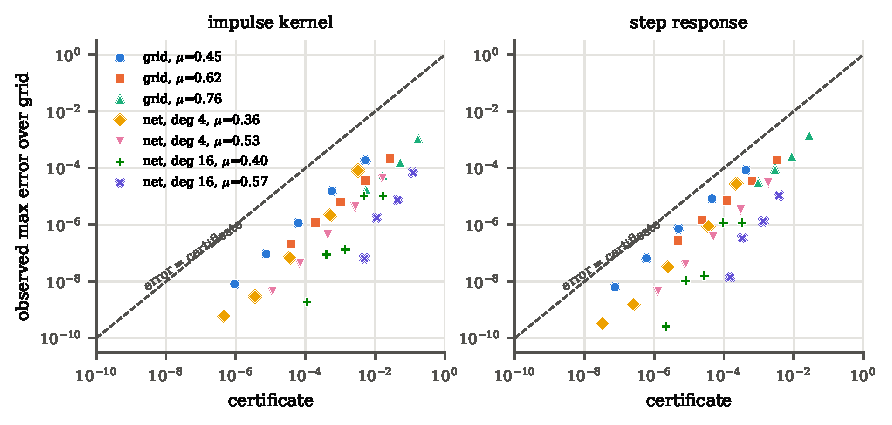
\includegraphics[width=\linewidth]{revision_assets/selected_responses_v13/f_59c757d49d52460d.pdf}
\caption{Observed maximum error over the time grid against the a posteriori certificate, for the impulse kernel (left) and the step response (right), over pruning thresholds $\tau=10^{-4}$ to $10^{-12}$. Points below the dashed line are certified. Grid: $301\times301$ thermal network; net: random network with $2^{16}$ states. Reference: \texttt{expm\_multiply} on the full matrix.}\label{fig:certificate}
\end{figure}

\subsection{Memory and time up to $2^{64}$ unknowns}\label{sec:scaling}
Figure~\ref{fig:scaling} fixes the query ($\tau=10^{-10}$) and varies $N$: the thermal grid from $10^4$ to $10^{12}$ states and the random network from $2^{16}$ to $2^{64}\approx1.8\times10^{19}$. The walk sum used 4.5~MiB for the whole process at every size, and took 0.07~s on the grid and 0.02~s on the network, visiting the same $\sim10^5$ walk prefixes regardless of $N$. The state-vector methods scale as they must. \texttt{expm\_multiply} took 0.5, 5.3, 50 and 634~s on the grid from $10^4$ to $10^7$ states, with 2.9~GiB at $10^7$, and 911~s and 1.3~GiB on the network at $2^{22}$; the Arnoldi method was slower still. Beyond these sizes the state vector alone exceeds the memory of the machine, and at $N=2^{64}$ it would require more than $10^{11}$~GiB. Where both ran, the results agreed to within a fraction of the walk sum's certificate.

\begin{figure}[t]
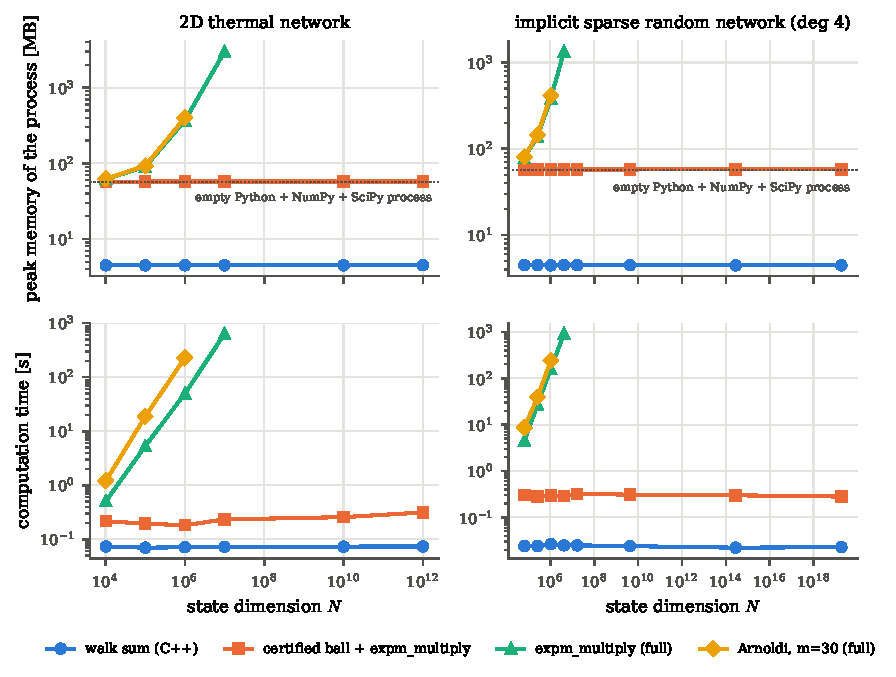
\includegraphics[width=\linewidth]{revision_assets/selected_responses_v13/f_7fd17134f08501c6.pdf}
\caption{Peak memory of the whole process (top) and computation time (bottom) against the number of unknowns, for the thermal grid ($\mu=0.45$) and the degree-4 random network ($\mu=0.36$) at fixed pruning threshold $\tau=10^{-10}$. Full-system methods were run up to $10^7$ (grid) and $2^{22}$ (network) states; beyond that their state vectors do not fit in memory. The dotted line marks the peak of a Python process that has imported NumPy and SciPy and holds no data.}\label{fig:scaling}
\end{figure}

\subsection{Stiffness}\label{sec:stiff}
Because the diagonal dynamics is integrated exactly, stiffness that resides in the diagonal barely affects the method. We drew the capacities of a $317\times317$ thermal grid log-uniformly over zero to three decades, which leaves the walk structure unchanged but increases $\|A\|_1$ from 26 to 19\,157. The walk sum visited the same 112\,429 prefixes in every case and took 0.08 to 0.16~s; the small increase comes from additional squaring levels in the kernel. \texttt{expm\_multiply} on the full grid went from 5.4 to 236~s, and the implicit BDF integrator, insensitive to stiffness, took 123 to 150~s at the matching tolerance.

\subsection{Many inputs and times for the price of one}\label{sec:batch}
On a network with $2^{18}$ states, one traversal produced the step kernel in 0.049~s, after which 100 zero-order-hold input waveforms of 20 random levels each were evaluated by discrete convolution in 0.013~s in total. Propagating the full state through the same waveforms with \texttt{expm\_multiply} took 47~s per waveform, and the two agreed to $4\times10^{-9}$. On a network with $2^{40}$ states, raising the number of output times from 10 to 1000 changed the traversal time only from 6~ms to 13~ms, and adding ramp, quadratic and exponential inputs to a step raised it from 5~ms to 8~ms.

\subsection{Comparison with local truncation}\label{sec:crossover}
A natural alternative is to integrate the system only on a set of states around the inputs. The bounds of Sec.~\ref{sec:error} certify such local truncations as well, which allows a comparison at equal guarantees. On random networks of degree 32 with $\mu=0.57$ and $2^{64}$ states, a certified step-response error of $10^{-4}$ took the walk sum 2.4~s and 6~MiB, including the search for the pruning threshold, against 13~s and 53~MiB for an adaptively grown local set and 1816~s and 3~GiB for a ball of radius 5 ($3.1\times10^7$ states); over nine combinations of graph realization and input location the adaptive set was 1.5 to 19 times slower. On a lattice the picture reverses: many walks revisit the same states, a local state vector merges them, and the local methods are orders of magnitude faster.

\subsection{Limitations}\label{sec:hard}
The cost of the walk sum grows steeply as the comparison ratio $\mu$ approaches one: on the thermal grid a certificate of $10^{-3}$ took $10^{-4}$~s at $\mu=0.45$, 42~s at $\mu=0.76$, and was not reached within 15~minutes at $\mu=0.87$. Directed transport with back-diffusion, which creates many excursions, and lightly damped oscillators over long horizons, whose walks cancel, are likewise expensive. The method is designed for systems whose local decay dominates the couplings, which is where it delivers certified answers in constant memory.

%% ---------------------------------------------------------------------------------------------
\section{Conclusion}\label{sec:discussion}

We have presented a method for linear differential equations that computes the requested outputs, for any number of input waveforms and observation times, without ever forming the state vector, and that certifies its truncation error. Its memory is independent of the number of unknowns: a few megabytes sufficed for systems with $2^{64}$ unknowns, far beyond what any state-vector method can hold, and its cost is insensitive to stiffness in the diagonal. The approach applies whenever the couplings and the local decay rates can be queried locally, as for discretized operators, network dynamics and master equations of stochastic processes. Tighter bounds on the discarded walks, which currently charge every walk as if it returned to the output, would translate directly into lower cost. Parametric sensitivities are also immediate, since the derivative of a walk factor with respect to a diagonal entry is one more appended node, and storing the solution on a small set of states near the inputs would trade memory for time continuously.

\paragraph*{Code and data availability.} The C++ implementation, tests, benchmark drivers and all measurement files from which the figures are generated are openly available at \url{https://github.com/itay-hen/pmrLTI}.

\begin{acknowledgments}
Research was sponsored by the U.S. Army Research Laboratory and was accomplished under Cooperative Agreement Number W911NF2410242. I.H. acknowledges support from the Office of Advanced Scientific Computing Research of the U.S. Department of Energy under Contract No. DE-SC0024389.
\end{acknowledgments}

\bibliography{revision_assets/selected_responses_v13/f_5297d78a43d37efd}
\end{document}
